\chapter{Evaluation}
\label{chap:eval}
In diesem Kapitel geht es um eine Evaluation der Idee, der verwendeten technologischen Prinzipien und deren Zusammenhänge zum methodischen Kontext. Dabei werden sowohl die Technologien, welche nun aktuell im Produkt verwendet werden, als auch jene, welche verwendet aber im Anschluss wieder ausgebaut wurden, beschrieben.

\section{Experiment: Reaktive Systeme}
Für den Kurs Reaktive Systeme wurde Lightbulb Learning für die Prüfungsvorbereitung der mündlichen Prüfung verwendet. Der Kurs bestand zu dem Zeitpunkt der Prüfung aus 7 Teilnehmern, welche in einem Zeitraum von 3 Wochen die Kursinhalte in Lightbulb Learning diskutieren konnten. Für die mündliche Prüfung wurden dann einige dieser Fragen verwendet, so dass die Prüflinge durch die Mitgestaltung der Fragen und Antworten und das Lernen dieser Fragen aktiv ihre Prüfungsergebnisse verbessern konnten. Dabei entstanden insgesamt 26 offene Fragen und 42 Antworten. Das Funktion zum Geben von Feedback wurde nicht genutzt. Eine Übersicht der Beiträge der Prüflinge ist in Abbildung \ref{fig:table} abgebildet.
\begin{figure}[H]
    \centering
    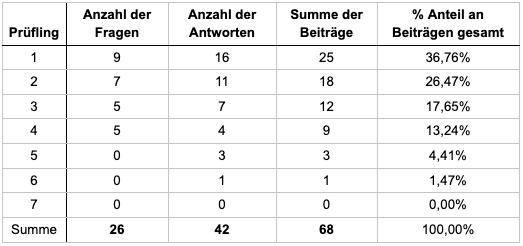
\includegraphics[width = .9\textwidth]{images/exrs.png}
    \caption{Darstellung der Anzahl der Beiträge gruppiert nach Prüfling}
    \label{fig:table}
\end{figure}
\noindent Es fällt auf, dass die Anzahl der Beiträge insgesamt nicht gleichverteilt sind, sondern wie in einer Pareto-Verteilung ein kleiner Teil der Studenten einen Großteil der Beiträge leistete und anders herum. Dies ist vermutlich durch die Freiwilligkeit bzw. die fehlende direkte Incentivierung bedingt, da die eigentliche Evaluation in der mündlichen Prüfung erfolgte. Etwa die Hälfte der Prüflinge zeigte durch die Involvierung in Diskussionen ihre intrinsische Motivation, und konnten diese Leistung zu ihrem Vorteil nutzen, wenn sie am Ende der Prüfung zwischen zwei Noten standen. In dem Fall wurde die Leistungsübersicht als weiterer Messpunkt für die Evaluation zurate gezogen. Schätzungsweise wäre das Ergebnis gleichverteilter ausgefallen, wenn der Lightbulb Learning Kurs als einziges Medium der Evaluation, wie beispielsweise bei Onlinekursen, genutzt werden würde. Dennoch gaben dieses Experiment bzw. die Teilnehmer des Kurses, auch neben den quantifizierbaren Größen geringer Messgröße, einige qualitative Hinweise auf die Benutzbarkeit der Software. Beispiele dafür waren das überflüssige Konzept der Entwürfe für Fragen, Antworten und Feedback, welches eher zur Verwirrung als zur Absicherung vor fälschlicherweise veröffentlichten Inhalten führte. Diese Funktion wurde daraufhin aus Lightbulb Learning herausgenommen. Ein anderer Einblick in die Perspektive mehrerer Benutzer war der Wunsch, gepostete Inhalte noch einmal anpassen zu können. Auch die Idee, bereits auf der Ebene der Frage die Anzahl der Antworten, und vielleicht sogar die richtige Antwort anzuzeigen, entstand in dieser Feedbackschleife. Auch der Login-Prozess, welcher den Zugriff auf die E-Mails auf dem jeweiligen Gerät voraussetzt, wurde kritisiert. Dieser Aspekt wurde durch die Integration des Logins mit GitHub als Authentifizierungsprovider adressiert. Somit verhalf dieses Experiment als erste breitere Anwendung des Systems und realistischen Bedingungen zu frühem, anwendbarem Feedback auf den Ebenen der Fachlichkeit und Technologie.

\section{Experimente mit AWS Lambda und Scala 3}
Während der Planung dieser Thesis war angedacht, in Scala 3 entwickelte AWS Lambda Funktionen für die Geschäftslogik zu verwenden. Dieses Vorgehen erwies sich als weniger effektiv als erwartet, so dass auch auf der Ebene der Technologieauswahl eine Kurskorrektur erfolgte. Die Gründe dafür sollen in diese Abschnitt beschrieben werden.
\subsection{Probleme mit AWS Amplify}
AWS Amplify\footnote{\url{https://aws.amazon.com/de/amplify/}} ist eine Werkzeugsammlung von AWS, welche sich die schnelle Entwicklung von Fullstack-Apps mit der AWS Cloud zum Ziel gesetzt hat. Überraschenderweise erwiesen sich diese Werkzeuge jedoch, aus einer Reihe von Gründen, als ungeeignet. Der wichtigste Grund war die Verwendung der aws-amplify Bibliotheken in Kombination mit dem Bundling Tool Vite\footnote{\url{https://vitejs.dev/guide/why.html}} für ES Modules, welches das Standardwerkzeug für das Bundling von SvelteKit-Applikationen ist. Die aws-amplify Bibliothek kann nicht mit Vite verwendet werden, da sie die veraltete CommonJS Struktur nutzt. Über einen konfigurativen Umweg mit manuellen Anpassungen an tieferliegenden technischen Schichten und dem Verzicht auf Vite war es dann möglich eine Svelte-App auf AWS Amplify zu deployen. Die Anforderung eines vollständigen Frontend-Frameworks, nämlich SvelteKit, konnte dadurch jedoch nicht mehr erfüllt werden. Diese Inkompatibilitäten werden regelmäßig in der Community diskutiert, wurden bisher aber noch nicht vom Provider aufgelöst. Hinzu kommt ein deutlich stärkeres Abhängigkeitsverhältnis zum Cloudprovider von AWS, der sogenannte Vendor Lock-in.
\subsection{Lambda Kaltstarts bei JVM-basierten Funktionen}
Als FaaS Dienst wurde AWS Lambda verwendet. Scala 3 Funktionen wurden als .JAR-Datei gebundlet und inklusive aller verwendeten Bibliotheken zu AWS hochgeladen. Ein Kaltstart tritt dabei immer dann auf, wenn der Container, in welchem die Funktion ausgeführt wird, vor der Ausführung erst gestartet werden muss. AWS macht keine genaue Angabe darüber, nach welcher Inaktivitätsdauer die Container heruntergefahren werden, empirische Erfahrungswerte schwanken in der Größenordnung einiger Minuten. Es gibt jedoch keine Garantie über die Dauer, über die ein Container mindestens aktiviert bleibt. Das bedeutet, dass jede Anfrage an eine Funktion einen Kaltstart darstellt, sofern nicht wenige Minuten vorher bereits eine Anfrage gemacht wurde. Der große Nachteil von JVM-basierten Funktionen wie etwa solchen, die in Scala 3 geschrieben sind, ist die Länge der Kaltstarts. Diese beträgt für einfache fachliche Funktionen mit wenigen einbezogenen externen Bibliotheken zwischen 25 und 40 Sekunden. Es gibt einige Lösungen für dieses (vorher bereits bekannte) Problem. Beispiele hierfür wären die Nutzung von Architekturmustern, welche die Asynchronität begünstigen, wie Command Query Responsibility Segregation \cite[vgl.][]{Fowler2011}, und Event Sourcing \cite[vgl.][]{Fowler2005} aus dem Umfeld des Domain-Driven Design \cite[vgl.][]{Evans2004}. Hier wird durch eine strikte Trennung zwischen Lese- und Schreibzugriffen (CQRS) und dem Persistieren von Serien von Events anstelle der aktuellen Zustände von beispielsweise Aggregaten (Event Sourcing) eine Systemstruktur etabliert, welche prinzipiell gut mit den durch Asynchronität erzeugten Latenzen zurecht kommt. Ein Beispiel für einen Aufruf in einem CQRS System ist in Abbildung \ref{fig:cqrs} dargestellt.
\begin{figure}[H]
    \centering
    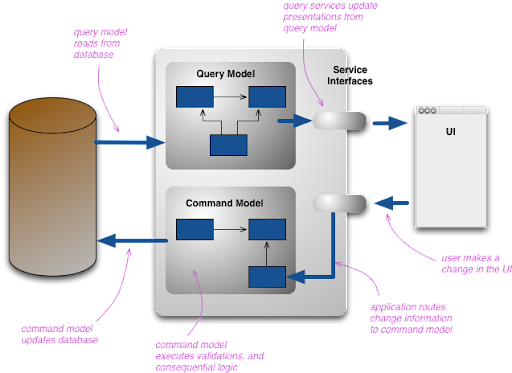
\includegraphics[width = .9\textwidth]{images/cqrs.png}
    \caption{Konzeptionelle Übersicht über einen Aufruf an ein CQRS System, \cite{Fowler2011}}
    \label{fig:cqrs}
\end{figure}
\noindent Der Aufruf beginnt unten rechts mit einem Nutzer, welcher über eine Benutzeroberfläche eine Änderung im System macht. Die Änderung wird an einen Endpunkt weitergeleitet, welcher ausschließlich für Schreibzugriffe genutzt werden kann. Der Endpunkt leitet die angeforderte Änderung an das Command Modell weiter. Dieses kennt die Validierungsregeln des Aggregats und etwaige Implikationen und Abhängigkeiten, so dass die Anfrage diesen Regeln folgend bearbeitet kann. Ist eine Anfrage fachlich gültig, so wird die Änderung an die Datenbank propagiert, und der Schreibzugriff ist vollständig. Der Lesezugriff wird davon getrennt aufgerufen, wofür ein Lesemodell (Query Model) benutzt wird. Die Struktur dieses Modells ist auf das Lesen optimiert, so dass hier effizient der aktuelle Zustand des Systems an den Benutzer zurückgegeben werden kann, selbst wenn ein Kaltstart darin enthalten ist. Der Kern dieser Idee beruht auf der Annahme, dass die meisten Applikationen deutlich häufiger Lese- als Schreibzugriffe durchlaufen, so dass eine Optimierung auf das Lesen mittels eines eigenen Lesemodells lohnenswert ist. Experimentell war es im Kontext von Lightbulb Learning grundsätzlich möglich, einige solcher eventbasierten Funktionen zu schreiben. Dennoch erwies es sich als sehr schwierig, im Zusammenspiel mehrer Funktionen, ein System zu gestalten, welches den in Kapitel \ref{sec:reqtools} beschriebenen Anforderungen an die Werkzeuge gerecht wird. Funktionen gehören per se keinen Gruppen zu, wie es beispielsweise Endpunkt zu Microservices tun, so dass eine strikte Aufrechterhaltung dieser Architekturprinzipien nicht intuitiv ist. Hinzu kommen die langen Kaltstarts, welche nicht mit den Standard Timeouts gängiger Browser von etwa 30 Sekunden vereinbar sind, sowie die damit verbundene katastrophale User Experience. Selbst wenn bei Schreibzugriffen das gewünschte Ergebnis zuerst angenommen werden kann, und im Fehlerfall durch eine verspätete Fehlermeldung dies korrigiert werden kann, so ist hierbei der Zusammenhang zwischen Handlung und Feedback so weit auseinander, dass eine Zuordnung für den Nutzer als schwierig gestaltet. Hinzu kommt, dass lesende Zugriffe zwar bereits in Aspekten der Datenstruktur und des zugehörigen Modells optimiert sind, eine Seite, die mehr als wenige Millisekunden lädt dabei allerdings nicht hinnehmbar ist. Somit kann man festhalten, dass die typischen eventbasierten Architekturmuster zwar durch ihre asynchrone Natur Latenzen abfedern können und für Systeme, in denen die Auslöser für Aufrufe keine Menschen sondern andere Systeme sind, geeignet sind. Für JVM basierte Lambdas reicht diese Federung für menschliche Nutzer allerdings schlichtweg nicht aus. Eine potentiell geeigneteres Architekturmuster für FaaS wird im folgenden Abschnitt beschrieben.
\subsection{FaaS API ist keine Aktoren API}
Während der Entwicklung des FaaS-basierten Ansatzes kam die Idee auf, dass Prinzipien wie sie im Aktorenmodell, bereits 1973 von Carl Hewitt \cite[vgl.][]{Hewitt1973} definiert wurden, für die Architekturgestaltung für FaaS basierte Systeme sinnvoll sein könnten, da es einige interessante Parallelen gibt. Im übertragenen Sinne würde dann eine Instanz einer FaaS-Funktion einer Instanz eines Aktors entsprechen. Wird ein Aktor aufgerufen, so kann er im wesentlichen Nachrichten empfangen, Berechnungen durchführen, eine Nachricht an einen ihm bekannten Aktor versenden, neue Aktoren erzeugen oder festlegen, wie er auf einen nächsten Aufruf reagieren wird \cite[vgl.][]{Hewitt2010}. Das Ziel dieser Struktur ist die Aufteilung der Anwendungslogik in kleinere, hierarchisch strukturierte und insbesondere leichtgewichtige Teilkomponenten mit eindeutig definierten Verantwortungsbereichen und Typen. Beispielsweise wirbt Akka\footnote{\url{https://akka.io/}}, einer Implementierung des Aktorenmodells von Lightbend\footnote{Interessanterweise ist einer der Co-Autoren des Reaktiven Manifests, Jonas Bonér, gleichzeitig auch der CEO von Lightbend und ursprüngliche Entwickler von Akka.}, mit ungefähr 2,5 Millionen Aktoren pro GB Heap-Speicher. Durch diese Eigenschaften eignen sich Aktoren als gute Grundlage für sehr stark skalierbare, reaktive Systeme (siehe Kapitel \ref{sec:res}). Würde es gelingen, eine Übersetzung dieser Prinzipien für das FaaS-Äquivalent zu entwickeln, so könnte möglicherweise ein noch weitaus skalierbareres System konstruiert werden. In diesem würde selbst das Aufsetzen der benötigten Infrastruktur außerhalb des Verantwortungsbereichs des Entwickler liegen. Das dafür erforderliche Framework könnte sich dabei hinsichtlich der API an der Aktoren API von Akka orientieren, wurde für Lightbulb Learning allerdings nicht tiefergehend verfolgt. Die Hauptgründe für diese Entscheidung war das fortwährende Problem der Kaltstarts sowie die (aktuelle) Schwergewichtigkeit von AWS Lambdas. Andere, leichtgewichtere FaaS Provider könnten sich in dieser Hinsicht als besonders durchsetzungsstark erweisen. Beispiele dafür sind Cloudflare Workers\footnote{\url{https://workers.cloudflare.com/}} oder Deno Deploy\footnote{\url{https://deno.com/deploy}}, welche durch andere Implementierung des FaaS Konzepts die Kaltstarts für ein vernachlässigbares Problem machen oder gar ganz lösen, während durch Deployments auf Edge Server \cite[vgl.][]{Meulen2018}, die Zugriffszeiten noch weiter verringert werden. Damit ist gemeint, dass Funktionen nicht nur auf einem oder weniger definierten Rechenzentren installiert und ausgeführt werden, sondern stattdessen weltweit verteilt sind. Dadurch können Nutzer immer auf das jeweils nächstgelegene Rechenzentrum zugreifen und somit die Netzwerklatenzen deutlich verkürzen. Eine detailliertere Bezugnahme auf Deno Deploy folgt im Ausblick.

\subsection{Libraries und Dokumentation für Java}
Ein weiteres Problem bei der Entwicklung von Scala 3 Lambdas war das geringe Vorhandensein von Dokumentation. Es gibt zwar für alle wesentlichen Schritte von der Entwicklung einer solchen Funktion, über das Einbinden von externen Bibliotheken und automatisierte Bereitstellen Anleitungen und Referenzen. Allerdings sind diese nicht offiziell von AWS und werden entsprechend nicht zwangsläufig aktuell gehalten, erfüllen nicht zwangsläufig einen Mindeststandard an Qualität und sind nicht unbedingt korrekt. Nachdem es dennoch gelungen war, Scala 3 Funktionen zu schreiben, zu deployen und aufzurufen, war ein weiteres Problem die Dokumentation des AWS-SDKs für Java\footnote{\url{https://aws.amazon.com/de/sdk-for-java/}}. Die Übersetzung von Java Konzepten auf Scala 3 Konzepte muss man selbst übernehmen. Dies ist nicht nur mit viel Aufwand verbunden, sondern hat auch zur Folge, dass die erwartete Schlankheit von funktionalen Programmen durch Übersetzungen zwischen diesen zwei Konzepten leidet.
\section{Svelte und SvelteKit}
\subsection{Intuitive Konzepte}
Die Entwicklung der Lightbulb Learning Applikation als transitionale App, welche die Vorteile von SPAs und MPAs kombiniert, erwies sich insgesamt als sehr produktiv und zielführend, auch wenn es einige Stolpersteine zu überwinden gab. Auch wenn vor der Entwicklung von Lightbulb Learning mit diesen Frameworks kaum Erfahrung vorhanden war, so konnten sich die wichtigsten Konzepte durch gute Dokumentation und eine hilfsbereite Community schnell angeeignet werden. Dabei ist insbesondere zu bemerken, dass sowohl Svelte als auch das Metaframework SvelteKit einige strukturelle Konzepte anwenden, welche der Intuition des Entwicklers entsprechen, ohne dabei bewusst diese Konzepte gelernt zu haben. Bei Svelte gehört dazu beispielsweise die Kombination aller semantisch zu einer Komponente gehörenden Styling-, Struktur- und Funktionselemente in einer einzigen Datei. Bei SvelteKit erfüllt das Dateisystemgestütze Routing diesen Anspruch, welches Entwicklern aus der klassischen MPA-Entwicklung bereits vertraut ist.
\subsection{Stolperstein: Serverseitige Authentifizierung}
Der bereits angedeuteten Stolpersteine sollte man sich jedoch auch bewusst sein, wenn man die Entscheidung für die Verwendung dieses Frameworks trifft. Ein Problem, welches bei der Entwicklung einer SvelteKit Applikation immer wieder auftaucht, ist der Mangel an externen Referenzen wie Tutorials, Codebeispiele und Bibliotheken, besonders im Vergleich zu Referenzen der aktuell gängigen Frameworks wie React, Angular und Vue. Ein besonders stark spürbares Beispiel ist das Nichtvorhandensein einer Bibliothek für die Serverside Authentifizierung mit Supabase. Diese ist zwar für Next.js und Nuxt bereits vorhanden, für SvelteKit bisher allerdings lediglich angekündigt \cite[vgl.][]{Schaeff2022}. Die aktuelle Alternative, eine eigene Implementierung, ist dabei hinsichtlich der hohen Komplexität und der damit verbundenen gelegentlichen Unzuverlässigkeit, nicht zufriedenstellend. Daher wird sie ersetzt, sobald eine offizielle Lösung veröffentlicht wird. Der aktuelle Ansatz basiert darauf, dass der Nutzer nach der initialen Authentifizierung das Access Token als Cookie bei jedem Request mitschickt, welches dann für die serverseitigen Prefetches wiederverwendet wird.
\subsection{NodeJS Laufzeitumgebung ist kein Browser}
SSR mit SvelteKit bedeutet, das Frontend-Code sowohl auf dem Server als auch auf dem Client ausgeführt wird. Auf dem Server wird dazu eine NodeJS-Umgebung verwendet. Allerdings unterscheiden sich diese Umgebung in mancherlei Hinsicht, so dass es sein kann, dass in den Code Weichen eingebaut werden müssen, welche das Verhalten abhängig von der jeweiligen Laufzeitumgebung beschreiben.
\subsection{PostgreSQL as a Service mit Supabase und lokale Entwicklung}
Die Entwicklung der Persistenzschicht mit Supabase erwies sich als pragmatisch, niederschwellig und zuverlässig. Dabei passte das Vorgehensmodell bei der Adaption dieses Dienstes gut zu den generellen Prinzipien bei diesem Produkt und der Serverless-Technologie allgemein. Zu Beginn wurde direkt auf der Webseite von Supabase ein Projekt angelegt und ein paar Tabellen generiert. Dabei konzentrierte sich der Lerneffekt insbesondere auf den Umgang mit der grafischen Benutzeroberfläche sowie einer Wiederauffrischung der Grundprinzipien des Umgangs mit PostgreSQL. Die erzeugten Tabellen waren vorerst vollständig öffentlich und es konnte ohne Authentifizierung auf diese zugegriffen werden. Daraufhin wurde die automatisiert provisioniert API vom Client aus konsumiert, um ein Gespür für den Umgang mit PostgREST und der inkludierten clientseitigen Bibliothek zu entwickeln. Anschließend folgte die Ersetzung des Login und Logout Features der Supabase Bibliothek, welche zur Reduktion der Komplexität vorerst ohne SSR die auf Amplify basierende Authentifizierung ersetzte. Nachdem es für Benutzer möglich war, sich zu Authentifizieren, war der nächste logische Schritt die Einbeziehung von RLS Regeln, welche den Zugang zu den Datensätzen hinter der API begrenzen. Mit diesem Vorgehen wurden noch einige weitere Schritte gemacht, bis hin zur Entwicklung mit einer lokalen Instanz von Supabase und der Versionsverwaltung der Datenbankstruktur in Form von Migrationsskripts, welche mittels der Supabase CLI angelegt, verwaltet und sogar auf die Produktivumgebung ausgerollt werden. Es zeigte sich, dass sich die Verwendung von Supabase aus der Perspektive eines Entwicklers sehr inkrementell gestalten lässt. Daher wird von einem frühen, funktionierenden Stand ausgegangen, und dieser kann schrittweise um viele weitere technische Schichten ergänzt werden, ohne dabei zu große Lernschritte vorauszusetzen. Der Umgang mit Supabase erwies sich durch die Kleinschrittigkeit und den inkrementellen Aufbau der Lernkurve als angenehm und für Projekte dieser Art als empfehlenswert.
\subsection{Serverless nur für CRUD-Szenarien?}
Eine verbreitete Ansicht ist, dass Serverless sich lediglich für Standardfälle wie CRUD (Create-Read-Update-Delete) Szenarien eignen würde, während bei komplexeren Anforderungen stets mehr Verantwortung über die Infrastruktur selbst übernommen werden müsse. Diese Ansicht kann mit Lightbulb Learning zwar nicht widerlegt werden, aber es soll als gutes Gegenbeispiel dienen. Es wurde bewusst darauf geachtet, dass möglichst viele unterschiedliche Anforderungsarten in der Implementierung berücksichtigt wurden. Das Ergebnis ist, dass es zu jedem Problem, für welches es ist in traditionellen Weltsicht eine Lösung gibt, auch in den Sphären der Serverless-Technologie ein äquivalente Lösung gab. So konnten, ohne einen einzigen Backendservice, einfache und komplexere logische Zusammenhänge abgebildet werden. Daten können langfristig, zukunftssicher und ohne Vendor-Lockin persistiert werden, es gibt öffentliche und private Daten und von letzterer Art kann die Datensicherheit und -integrität gewährleistet werden. Auch das Hosten der Webseite, die Ausführung von Funktionen auf der Datenbank, die Build-Pipeline und die Versionsverwaltung des Quellcodes kommen ohne eigene infrastrukturelle Verantwortung aus. Der Querschnitt von Funktionen, welcher sich über mehrere technische, gestalterische und geschäftliche Schichten erstreckt, konnte von einem einzigen Entwickler vollständig in dem Zeitraum der Thesis umgesetzt werden. Lightbulb Learning wird nun von einigen Professoren und Studenten an der eigenen Hochschule verwendet, und es wurde Interesse an dem Produkt von einem wissenschaftlichen Mitarbeiter der Pädagogischen Hochschule Karlsruhe bekundet.

\section{Serverless-Prinzipien}
Drei Prinzipien, die alle Serverless-Technologien gemeinsam zu haben scheinen, sollen in diesem Absatz zusammengefasst werden. Diese lauten

\begin{enumerate}
    \item Abstraktion
    \item Delegation
    \item Fokus
\end{enumerate}

\noindent und stehen im folgenden Abhängigkeitsverhältnis zueinander. Technische Herausforderungen, wie beispielsweise der Betrieb einer Datenbank, werden abstrahiert. Das bedeutet beispielsweise, dass die Verwaltung der benötigten Infrastruktur automatisiert wird. Durch diese Abstraktion wird die Delegation möglich. So kann beipielsweise durch die zur Verfügungstellung einer entsprechenden Schnittstelle ein Nutzer die abstrahierte technologische Herausforderung als Dienstleistung nutzen, und dadurch Aufwand sparen. Zusätzlich können meta-Herausforderungen wie Skalierbarkeit und Elastizität in einer Dienstleistung mitinbegriffen sein. Das möglicherweise entstehende Abhängigkeitsverhältnis muss, insbesondere aus der Perspektive des Nutzers einer solchen Dienstleistung, bewusst gehandhabt werden. Gerade in einer frühen Produktphase, in welcher der Fokus auf der Evaluations einer Produktidee liegt, sind die Vermeidung solcher Abhängigkeiten mit hohem Aufwand verbunden. Durch die Delegation der genannten technischen Schichten erhöht sich somit der Fokus der Entwicklung auf das Geschäftsmodell. Dies hat Einfluss auf angrenzende Bereiche, wie in den Kapiteln \ref{sec:leansl} und \ref{sec:agilesl} diskutiert wird: Ideen können früher evaluiert werden, und die Iterationszeit durch den Build-Measure-Learn Zyklus lässt sich verkürzen.